\begin{figure}[ht!]
  \centering
%   \begin{minipage}[b]{\linewidth}
%   \centering
  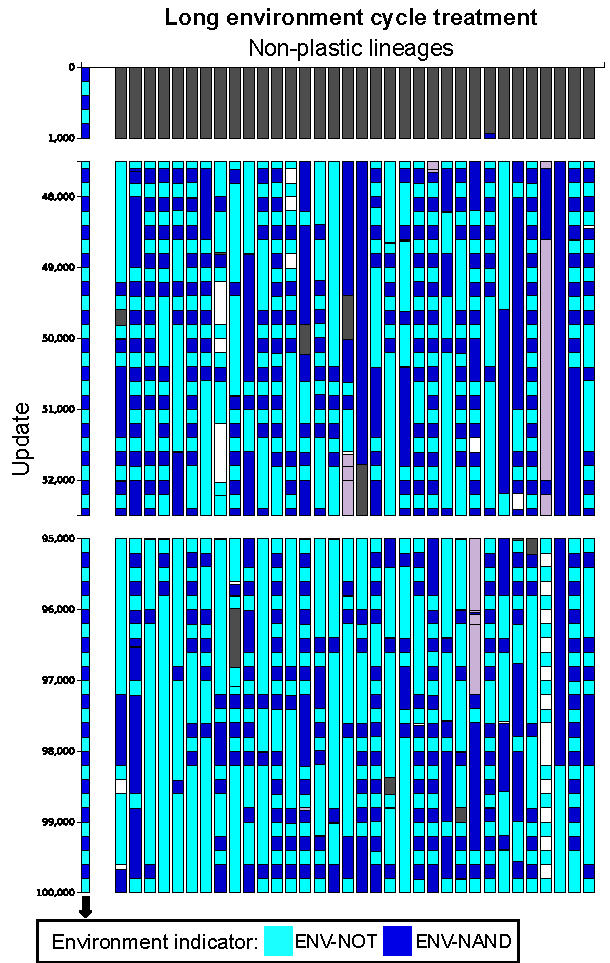
\includegraphics[height=0.65\textheight, keepaspectratio]
  {chapters/02-evolutionary-origins-of-plasticity/media/long-cycle-non-plastic-lineages.pdf}
  \caption{\small 
  \textbf{Time-sliced lineage visualization of non-plastic, dominant genotypes from the long environment cycle treatment.}
  Abbreviated color reference: 
  cyan represents unconditional NOT task performance, 
  dark blue represents unconditional NAND task performance, 
  light purple represents sub-optimal forms of plasticity,
  and dark purple represents optimal plasticity. 
  Refer to Figure \ref{chapter:origins-of-plasticity:fig:task-profiles} for a full legend of phenotype colors.
  }
  \label{chapter:origins-of-plasticity:fig:long-cycle-lineages}
%   \end{minipage}
\end{figure}
